\section{Result and Discussion}

In this work, we propose to use an artificial neural network as an alternative
way to compute the strength ratio of composite material instead of a two-step
procedure, based on classical lamination and failure theory.
Fig. \ref{fig:ga_nn} shows the changes of the fitness and error during the
evolution procedure. The fitness is obtained through the performance estimation
technique of an artificial neural network. As shown in this figure, fitness
grows during the initial stage; then, it slowly converges as generation
proceeds. It implies genetic algorithm can find a better artificial neural
network with the evolution of the number of neurons in the hidden layer,
connection relationship, activation functions, and connection weights.

\begin{figure}[!tb]
	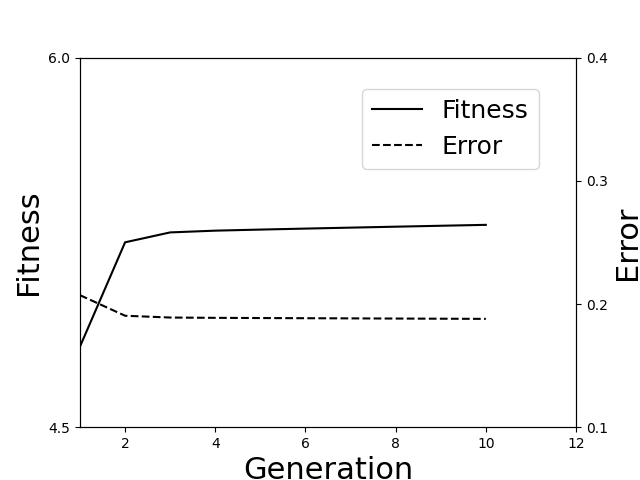
\includegraphics[width=0.9\linewidth]{./fig/result_ga_ann.png}
	\caption{Fitness and averaged sum-of-squares errors of the pre-trained artificial neural network as generations proceed.}
	\label{fig:ga_nn}
\end{figure}

\begin{figure}[!tb]
	\centering
	\def\svgwidth{\columnwidth}
	\import{fig/}{post_train.pdf_tex}
	\caption{The illustration of the behaviour of fitness on the training dataset during the training session.}
	\label{fig:final_train}
\end{figure}


Fig. \ref{fig:final_train} shows the rest training of the artificial neural
network obtained by the GA. After the optimizing process, we get the best
individual, which is a pre-trained neural network. We continue to train it with
a standard gradient-based descent algorithm. The target neural network
converges rapidly at first, and further training doesn’t reduce the error
efficiently.  Then, we use the target ANN to predict the properties of
laminated composite material.

\begin{table}	
	\centering
	\caption{Comparsion between practical and simulation}
	\label{tab:simu}
		\resizebox{\textwidth}{!}{
	\begin{tabular}{cccc|cc|cc}
		\toprule
		\multicolumn{4}{c}{\textbf{Input}} &  \multicolumn{4}{c}{\textbf{Output}} \\
		\midrule
		Load  &  \makecell{Laminate \\ Structure }  & \makecell{Material \\ Property} & \makecell{Failure \\  Property}  &
		\multicolumn{2}{c}{ \makecell {CLT \\MS  Tsai-Wu}} & \multicolumn{2}{c}{ \makecell {ANN \\MS  Tsai-Wu}}\\
		\midrule
		-10,40,20  &  26,-26,168,1.27 & 116.6,7.67,0.27,4.17 & 2062.0,1701.0,70,240,105 & 0.342 & 0.476 & 0.351 & 0.492 \\
		20,-70,-30 &  10,-10,196,1.27 & 181.0,10.3,0.28,7.17 & 1500.0,1500.0,40,246,68  & 0.653 & 0.489 & 0.612 & 0.445 \\ 
		60,-20,0   &  82 -82,128,1.27 & 181.0,10.3,0.28,7.17 & 1500.0,1500.0,40,246,68  & 1.663 & 0.112 & 1.673 & 0.189 \\
		\bottomrule
	\end{tabular}
	}
\end{table}

To present the evaluation result of the ANN straightforwardly, we randomly
select several experiment results from the validation dataset, as is shown
in Tab. \ref{tab:simu}.  Comparing the strength ratio outputs based on CLT and
ANN from Tab. \ref{tab:simu}, we can see that the calculation of strength ratio
can be achieved using a two-layer neural network, without the intensive
computation of matrix multiplication.





